\documentclass[12pt,fleqn]{exam}
\usepackage{pifont,bbding,url}
\usepackage{dingbat}
\usepackage{amsmath}
\usepackage{centernot}
\usepackage{fleqn}
\usepackage{epsfig}
\usepackage{pdfpages}
\usepackage{fourier} %{mathptm}
\usepackage[activate={true,nocompatibility},final,tracking=true,kerning=true,spacing=true,factor=1100,stretch=10,shrink=10]{microtype}
\usepackage{xcolor}
\usepackage{enumerate}
\usepackage{tcolorbox}
\usepackage{mathtools}
\DeclarePairedDelimiter\ceil{\lceil}{\rceil}
\DeclarePairedDelimiter\floor{\lfloor}{\rfloor}
\DeclarePairedDelimiter{\parens}{\lparen}{\rparen}

\usepackage[letterpaper, margin=0.75in]{geometry}
\usepackage{amssymb, enumerate}
\shadedsolutions
%\definecolor{SolutionColor}{rgb}{0.9,1,1}
\definecolor{SolutionColor}{rgb}{1,1,0.7}
\addpoints
\boxedpoints
\pointsinmargin
\pointname{pts}

\newcommand{\dotprod}{\, {\scriptzcriptztyle \stackrel{\bullet}{{}}}\,}
\begin{document}

\newcommand{\reals}{\mathbf{R}}
\newcommand{\integers}{\mathbf{Z}}
\newcommand{\bi}{\mathbf{i}}
\newcommand{\bj}{\mathbf{j}}
\newcommand{\bk}{mathbf{k}}

\newcommand{\Mod}[1]{\ \mathrm{mod}\ #1}
\newcommand{\ex}{I}
\newenvironment{alphalist}{
  \begin{enumerate}[(a)]
    \addtolength{\itemsep}{-1.0\itemsep}}
  {\end{enumerate}}

\newenvironment{handlist}{
  \begin{enumerate}[\leftthumbsup]
    \addtolength{\itemsep}{-1.0\itemsep}}
  {\end{enumerate}}

\large
\vspace{0.1in}
\noindent\makebox[3.0truein][l]{{\bf MATH 250}}
{\bf Name:}\hrulefill\\
\noindent \makebox[3.0truein][l]{\bf Exam \ex \/}
{\bf Row:}\hrulefill\

\large

\vspace{0.1in}

\noindent Exam \ex\/  has questions 1 through  \numquestions \/ with a total of \numpoints \/ points.  This exam is printed on both sides of the paper.

\noindent \begin{tcolorbox}
\begin{minipage}{6.5in}
\begin{enumerate}

\normalsize 
\item \textbf{Show all of your work.} Do not expect to earn full credit for a correct answer without the needed work.

\item Divine intervention is \emph{not} a substitute for showing your work.

\item If your answer is wrong, but your work shows me that you know the major steps in solving a problem, you will likely earn
some partial credit.

\item Your work should convince me that not only could you correctly solve the given 
problem, but you could also solve any related problem.

\item If a question asks for a sentence, write your answer as an English sentence. 

\item No talking, no sharing calculators, and no scratch paper.
\item  Turn your phone off and put it out of sight.
\item  Clear your desk of everything, except a pencil, eraser, and a calculator.
\item If you never make a mistake, you may use ink; otherwise use a pencil.
\item Do not unstaple the pages of your exam.
\item We'll all start at the same time--it's the polite thing to do.
\item Write your answers in the space provided. 
\item If you do not want something graded, erase it or clearly cross it out. 
\item You may stare at your feet, your paper, or the ceiling, but nowhere else. 
\item If you wear a  baseball cap, wear it backwards so I can see your eyes.
\item Work each problem correctly.
\item When you are finished, collect your things, place your exam paper in the folder on the front desk,
and quietly leave the room.
\item After you turn in your paper, I will not answer questions about the test until after it is graded.

\item Read all directions and problems carefully. 
\end{enumerate} 
\end{minipage} 

\end{tcolorbox}

\newpage
\begin{questions}

\question True or False:

\begin{parts}

 \part [5] \underline{$\phantom{xxxxxx}$}  $\varnothing = \{\varnothing \}.$
 \part [5] \underline{$\phantom{xxxxxx}$}  $\varnothing \subset \{\varnothing \}.$
 \end{parts}
 
 \question [10] Write the \emph{contrapositive} of the statement
    \emph{If an integer $n$ is even, then $2 n +  2$ is even.}
\begin{solution}[2.2in]
\end{solution}

 \question [10] Write the \emph{converse} of the statement
 \emph{If an integer $n$ is even, then $2 n +  2$ is even.}
\begin{solution}[2.2in]
\end{solution}

\question [10] Give an example of a \emph{conditional statement that is true}, but whose converse is false.
\begin{solution}%[2.2in]
\end{solution}
 
 \newpage
\question Enumerate the members of each set:

\begin{parts}

\part [10]  \( \{1,2,\sqrt{5} \} \cap \{1,2, \sqrt{2023}\} \)
\begin{solution}[1.5in]


\end{solution}
\part [10]  \(  \{1,2,\sqrt{5} \}  \cup \{1,2, \sqrt{2023}\} \)
\begin{solution}[1.5in]
\end{solution}

\part [10]  \(  \{1,2,\sqrt{5} \}  \setminus \{1,2, \sqrt{2023}\}  \)
\begin{solution}[1.5in]
\end{solution}
\end{parts}


\question [10] Using a truth table, show that \mbox{\(P \implies Q\)} is logically equivalent to \mbox{ \(\lnot Q \implies \lnot P\)}.
\begin{solution}%[2.50in]

\end{solution}

\vfill
\newpage
 
 \question [10] Let $A$ and $B$ be sets. Write the \emph{contrapositive} of the statement $A \setminus B  = A \implies A \cap B = \varnothing$.
 

 \begin{solution}[2.50in]

\end{solution}

\question [10] Let $A$ and $B$ be sets. Show that $\left(A \subset B \right) \land \left(B \subset C \right)  \implies A \cap C$. I've started the proof for you

\textbf{Proof} Suppose $x \in A$; we'll show that $x \in C$.  



\vfill 

\end{questions}
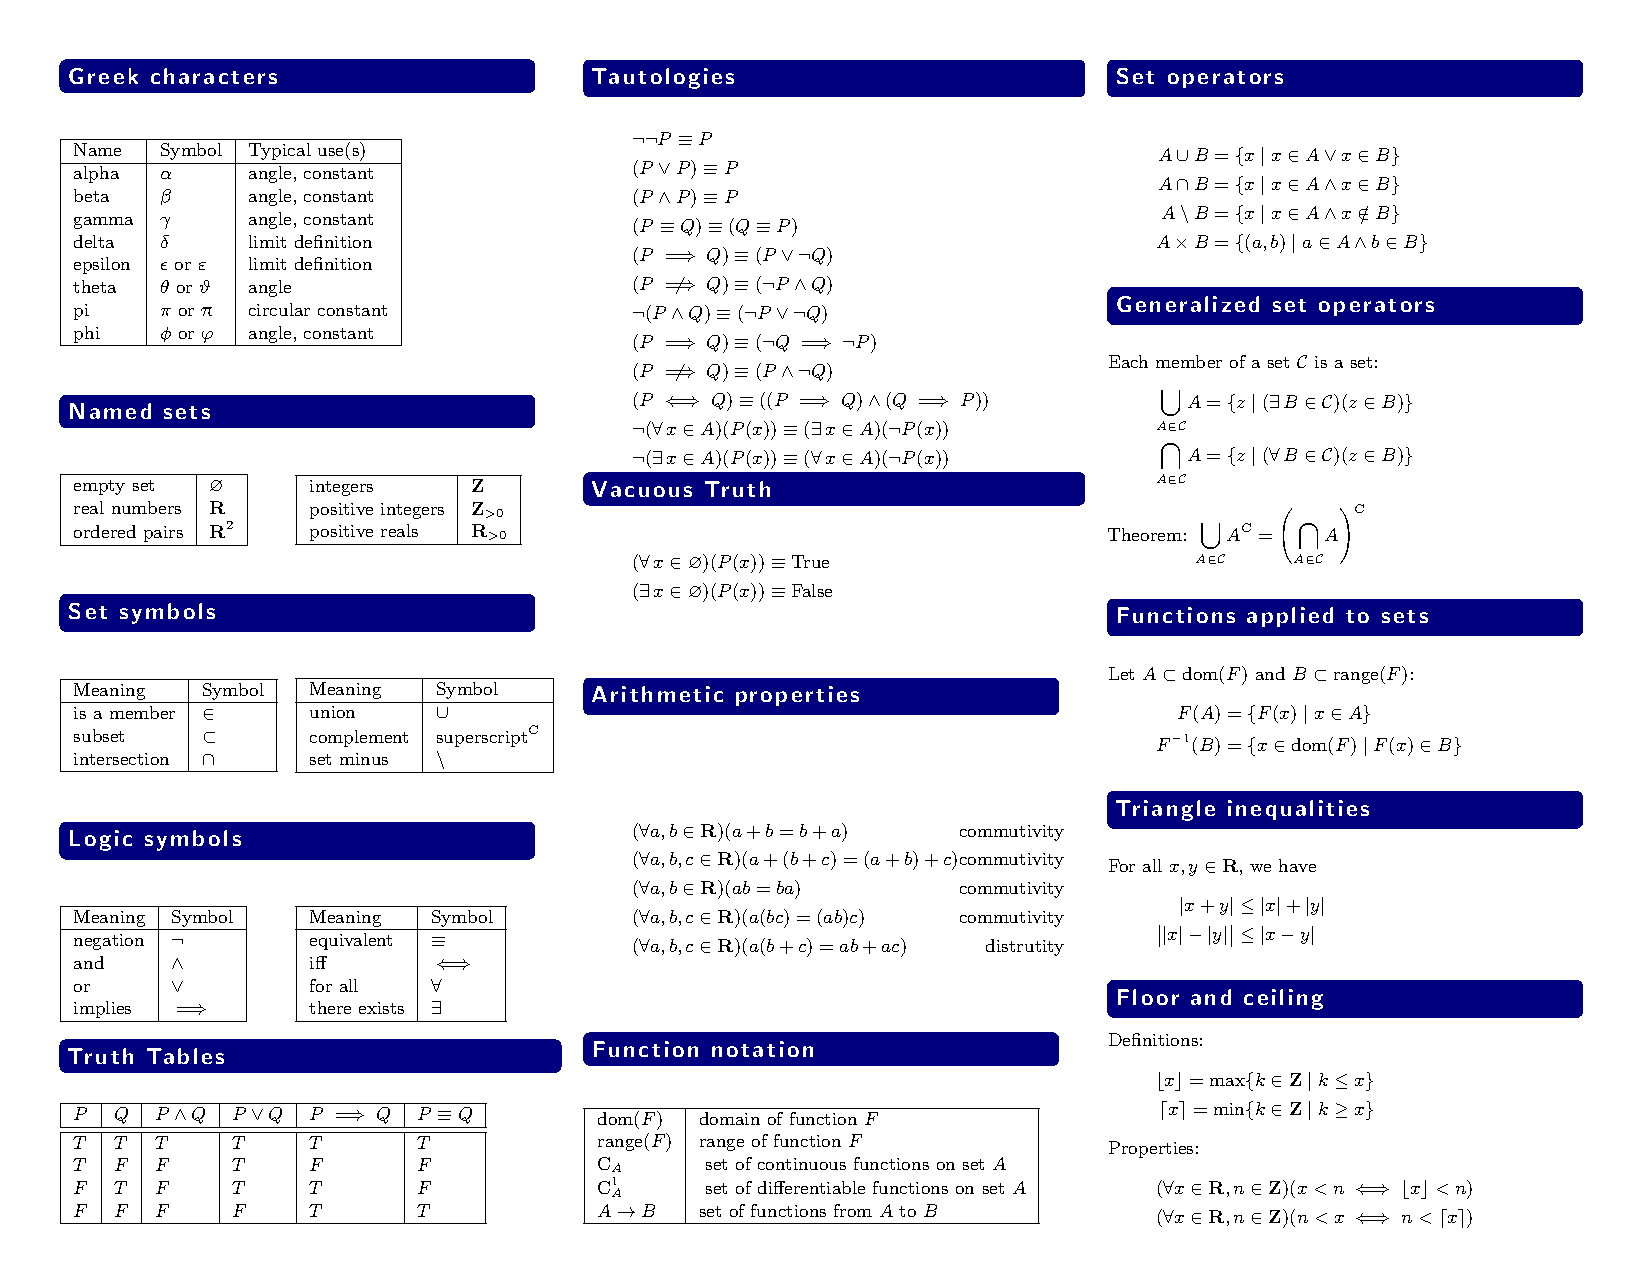
\includepdf{foundations-of-math-quick-reference}
\end{document}